\subsection{\ac{SDS} components}\label{sds_button}
An essential part of the implementation of a design system is the components. As described in chapter \ref{sds-component}, the design system builds its components using the Lit framework. This chapter presents an example of the button component of the \ac{SDS}. In addition, it shows a complete example of a component constructed with design tokens and documented with the Storybook.  \\
The components use TypeScript to take advantage of custom decorators. The decorators provided by Lit further simplify the boilerplate code for creating a web component. \\
\lstinputlisting[linerange={1-4},firstnumber=1,caption={Initialization of \ac{SDS} button component},label=ButtonInit]{../Code/src/components/button.component.ts}
In listing \ref{ButtonInit}, the \texttt{@customElement} decorator initializes the component by passing the tag name as a string and appending it to an \ac{ES6} class. For it to work correctly, the class must extend the Lit Element class. Finally, the web component registers itself, and users can use the component with the defined tag, in this case \texttt{<saas-button>}. \\
In order to see something when the web component just created is used, it must implement the render method. This method expects a \texttt{TemplateResult}. 
\lstinputlisting[linerange={19-26},firstnumber=19,caption={Rendering of \ac{SDS} button component},label=ButtonRender]{../Code/src/components/button.component.ts}
Lit element provides the import of an \texttt{html} string literal that constructs the \texttt{TemplateResult} expected by the render function. With this functionality, Lit provides an efficient way to respond to variable changes and intelligently update the \ac{DOM}. \\
Properties also use custom decorators and declare properties on web components by writing \texttt{@property} in front of a class attribute (line 19-20, Listing \ref{ButtonRender}). Thus, Lit Element implements change detection and add automatic type conversion. For a detailed description of the capabilities of this decorator, see the documentation. The property value of the created button web component changes and the constructed template string reacts to these changes and updates the displayed template accordingly. \\
Last but not least, the web component must use the defined design tokens. Since \ac{CSS} variables define these tokens, components consume them as follows: 
\lstinputlisting[linerange={5-20},firstnumber=5,caption={Styles of \ac{SDS} button component},label=ButtonStyles]{../Code/src/components/button.component.ts}
The Lit framework implements a static property of the \texttt{styles} of its classes. The component uses a literal \texttt{css} string to convert a string into the required \texttt{CSSResult} type. This way, it would be possible to consume design tokens via input properties. However, to manipulate design tokens in one place, the components of \ac{SDS} will use \ac{CSS} variables. It is possible to customize specific tokens throughout the design system by adapting them. Each component in the \ac{SDS} will use the defined tokens. Line 7-9 in listing \ref{ButtonStyles} shows an example of design tokens for the button component in the \ac{SDS}. \\
Finally, the button component is displayed in Storybook, the documentation tool for \ac{SDS}. Due to the limited time frame of this elaboration, the documentation is kept short. Figure \ref{storybook_button} is an example of the documentation of \ac{SDS} components. As in other mature design systems, the subsequent development of \ac{SDS} will add a full version of the documentation. \\
\begin{figure}[htbp]
    \centerline{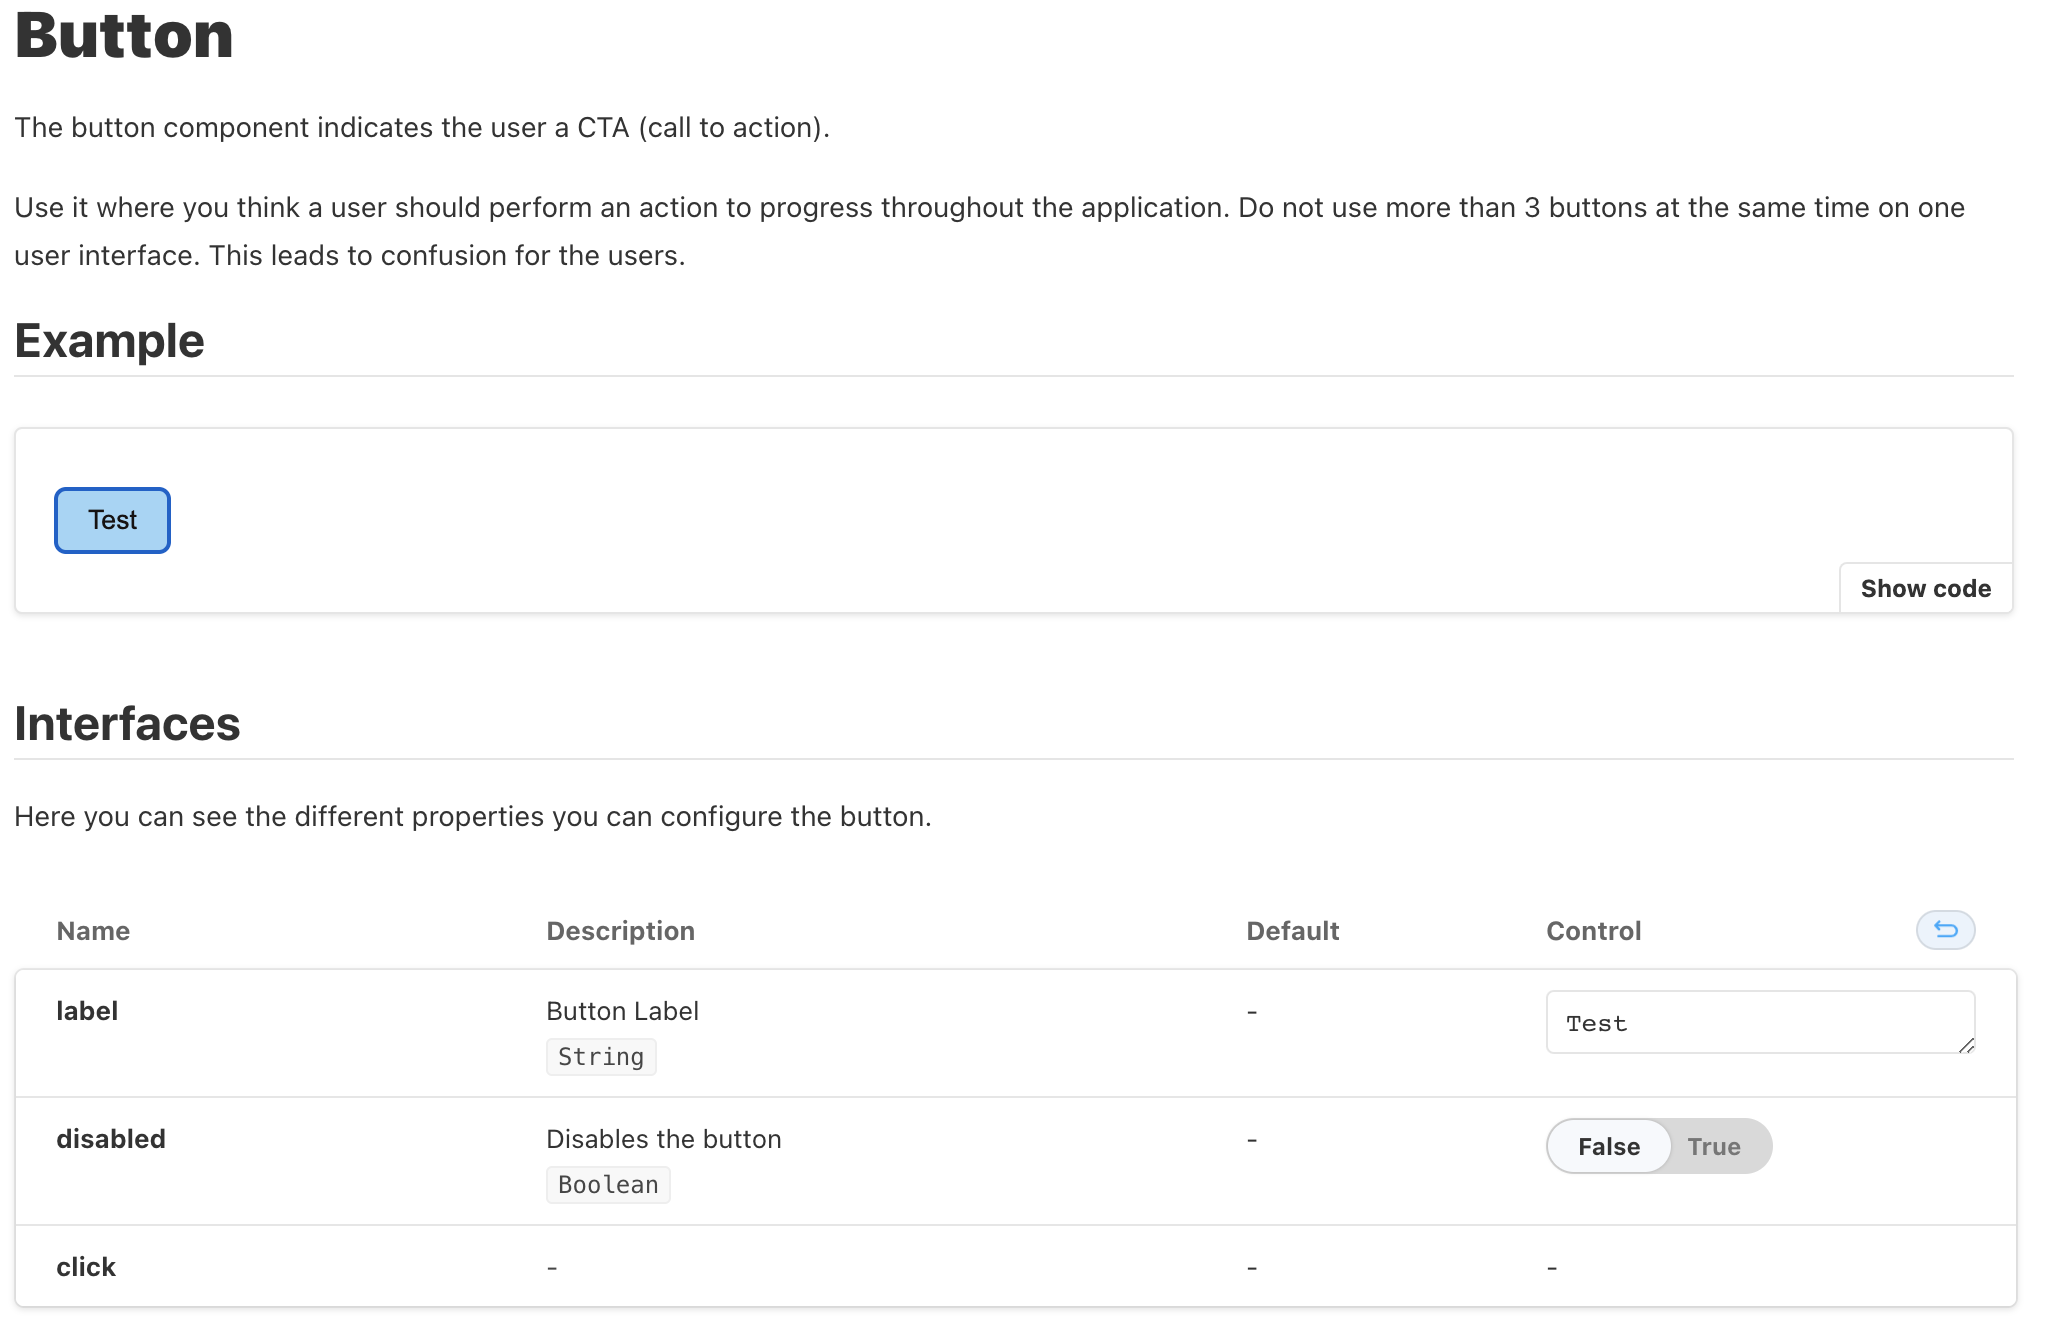
\includegraphics[width=\linewidth]{images/storybook_button.png}}
    \caption{Example documentation of the \ac{SDS} button component}
    \label{storybook_button}
\end{figure}
At the moment, the documentation consists of a short description that briefly explains to the developer how and where he can use the button in his applications. In addition, a live example of the component is presented, automatically linked to the properties shown below. When the properties are changed, the example above is updated. This instant feedback gives developers or designers who want to use this component the chance to determine which configuration is most suitable for their use cases. \\
Inspecting the \ac{DOM} element of the button component, the element explorer looks like Figure \ref{button_element_explorer}. The new web component, the \texttt{saas-button}, is a valid \ac{DOM} element. A new shadow root is opened inside the button component. For this, the button component opens a new shadow root. The shadow root allows the web component to isolate styles and elements from the global document. The button component defines the elements used to display in this shadow root. Also, the code defines the styles for the button at the shadow \ac{DOM} level, so the rest of the \ac{DOM} tree never receives these styles. This technique helps to keep elements and styles separated and easy to understand. \\
\begin{figure}[htbp]
    \centerline{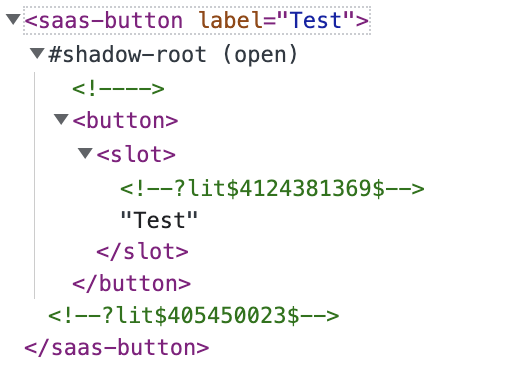
\includegraphics[height=100px]{images/button_element_explorer.png}}
    \caption{Inspection of \ac{SDS} button in element explorer}
    \label{button_element_explorer}
\end{figure}
It is crucial to declare that \ac{CSS} variables in the document's root are also available in the shadow \ac{DOM}. In contrast, style declarations, e.g., for the button element in the overall document, are not applied to \ac{DOM} elements in the shadow \ac{DOM}. \\
The \texttt{<slot>} element in the shadow \ac{DOM} is a default placeholder for anything inserted into the \texttt{<saas-button>} element when using the web component. The content is projected within the shadow \ac{DOM} and inserted in the place of the \texttt{<slot>} element. Slots make it possible to create nested elements with web components which is helpful in many different use cases.  \\

The example of a simple button component shows how to create and use the components of \ac{SDS}. From here, building all the different components needed to create patterns is trivial. The building is simple because patterns, as described, are a combination of components that applications reuse. The missing piece to using the \ac{SDS} in an application is integration, which the next chapter explains.